\documentclass{article} % For LaTeX2e
\usepackage{nips13submit_e,times}
\usepackage{hyperref}
\usepackage{url}
\usepackage{tgtermes}
\usepackage{graphicx} % Required for including pictures
\usepackage{wrapfig} % Allows in-line images
\usepackage{amsmath}
\usepackage{amssymb}
\usepackage{booktabs}
\usepackage{amsthm}
\usepackage{algorithm}
\usepackage{caption}
\usepackage{cmap}
%\documentstyle[nips13submit_09,times,art10]{article} % For LaTeX 2.09


\title{Machine Comprehension using Improved Bi-Directional Attention Flow Network}


\author{
Sijun He \\
Stanford University \\
\texttt{sijunhe@stanford.edu} \\
\And
Jiajun Sun \\
Stanford University \\
\texttt{jiajuns@stanford.edu} \\
\And
Mingxiang Chen \\
Stanford University \\
\texttt{ming1993@stanford.edu} \\
}

% The \author macro works with any number of authors. There are two commands
% used to separate the names and addresses of multiple authors: \And and \AND.
%
% Using \And between authors leaves it to \LaTeX{} to determine where to break
% the lines. Using \AND forces a linebreak at that point. So, if \LaTeX{}
% puts 3 of 4 authors names on the first line, and the last on the second
% line, try using \AND instead of \And before the third author name.

\newcommand{\fix}{\marginpar{FIX}}
\newcommand{\new}{\marginpar{NEW}}

\nipsfinalcopy % Uncomment for camera-ready version

\begin{document}


\maketitle

\begin{abstract}

\end{abstract}

\section{Introduction}
\label{introduction}

Almost all human knowledge are recorded as text. The ability to read, understand and extract information from text is natural for human beings, but very challenging for machines. In recent years, the field of Machine Comprehension (MC) has made significant progress. Many end-to-end neural network systems have gained tremendous success on the task of Question Answering (QA), where the machines answer questions, using words contained within the given related context. Many of the success can be attributed to the invention of the attention mechanism, which allows the system to focus on specific area, may it be a sentence in a paragraph, or a selected region of pixels in an image. The leading models on the Stanford Question Answering Dataset (SQuAD) (Rajpurkar et al. 2016) , such as Dynamic Coattention Networks (Xiong et al. 2017) and Bi-Directional Attention Flow (Seo et al. 2017), all involves innovation on their attention mechanisms in the architecture. 

The objective of our project is to propose a filtering layer in the multi-layer hierarchical neural network architecture that can potentially enhance the performance of the attention mechanism. The filtering layer is inspired by the concept of similarity from collaborative filtering in recommendation systems and aims to amplify the hidden signal of relevant information while filtering out the redundant information. Our preliminary experimentation on the Stanford Question Answering Dataset (SQuAD) shows that the filtering layer can effectively assist the attention layer in Bi-Directional Attention Flow (BiDAF).
\section{Models}
\label{models}

Our neural network architecture (Figure 1) has six layers, of which four are identical to the BiDAF model and one is slightly modified. The remaining one is the filtering layer.
\begin{enumerate}
\item \textbf{Word Embedding Layer} maps each word to a high-dimensional representation using a pre-trained GloVe (Pennington et al.) word embedding model.
\item \textbf{Filtering Layer} filters the redundant information and emphasizes on the most relevant context
\item \textbf{Contextual Embedding Layer} models the contextual representation of words in its surrounding neighborhood
\item \textbf{Attention Flow Layer} intertwine the contextual representation of words in the question and the context into a question-aware representation for each word in the context
\item \textbf{Modeling Layer}  captures the interaction among the question-aware representation of words in the context
\item \textbf{Output Layer} outputs the answer
\end{enumerate}
\subsection{Word Embedding Layer}

The word embedding layer maps each individual word into a high-dimension vector space. It is a set of pre-trained GloVe (Pennington et al.) word vectors using datasets provided by Wikipedia 2014 and Gigaword 5. The dimensionality of the vectors $d$ is 100. The word embedding layer outputs the context representation $\textbf{X} \in \mathcal{R}^{d \times T}$, where $T$ is the maximum number of context length and $ \textbf{Q} \in \mathcal{R}^{d \times J}$, where $J$ is the maximum number of question length.

\subsection{Filtering Layer}

The filtering layer is inspired by Wang et al. (2016) and the concept of similarity of collaborative filtering in Recommendation Systems. The idea is that only a small portion of context is needed to answer the question so we use the cosine similarity to dampen the signal of redundant information. For each word pair with context word $x_i \in \textbf{X}$ and $q_j \in \textbf{Q}$, we compute the cosine similarity
$$\text{sim}_{i,j} = \frac{x_i^T q_j}{|x_i||q_j|}$$
And the relevancy is computed as a weighted average of the cosine similarity, with $W_{\text{sim}}$ as a trainable weights of $\mathcal{R}^{J}$.
$$r_i = W_{\text{sim}}^T\left[\text{sim}_{i,:}\right]$$


\subsection{Contextual Embedding Layer}

We use a Bi-directional Long Short-Term Memory (LSTM) (Hochreiter et al.) network as our encoding layer. Contexts and questions will be fed into the network respectively, while the output from each hidden state are all be recorded. Note that the output of which will be $2d$-dimension vectors (where $d$ is 100 in our model) due to the concatenation of two output for both direction of the network.

\begin{figure}[h]
\begin{center}
%\framebox[4.0in]{$\;$}
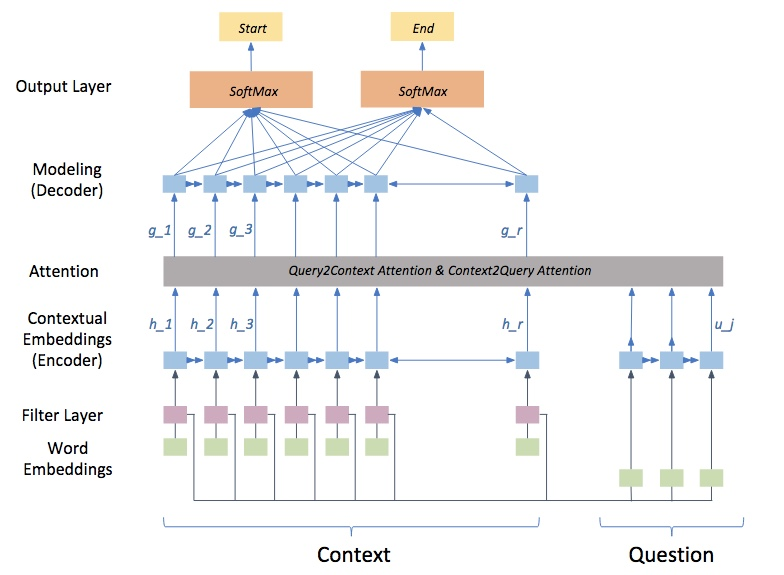
\includegraphics[width=0.9\textwidth]{withfilter.jpeg}
\end{center}
\caption{Bi-Directional Attention Flow Model }
\end{figure}

\subsection{Attention Flow Layer}

The attention layer is used to couple the information from the question and the information given by the context. It categories the importance of the attention to each word vector in the text (both contexts and questions). The input of this layer is contextual vector of the context $\textbf{H}$ and the question $\textbf{U}$.

In this layer, the attention is calculated from the similarity matrix of $\textbf{H}$ and $\textbf{U}$ as follow:\\
\newline
\centerline{$\textbf{S}_{ij}=\alpha (\textbf{H}_{:,t}, \textbf{U}(:,j))$}\\
\newline
where $\textbf{S}_{ij}$ indicates the similarity of the word i in the context and the word j in the query, and $\alpha$ is the bilinear factor introduced by Chen et al. (2016) which is defined as\\
\newline
\centerline{$\alpha (h,u)=h^T\textbf{W}_{\text{bi}}u$}\\
\newline
$\textbf{W}_{\text{bi}}$ is a trainable matrix of $\mathcal{R}^{2d\times 2d}$. The similarity matrix is different from the original BiDAF model where they used 
$$\alpha (h,u)=\textbf{W}_{\text{bi}}^T[h; u; h \circ u]$$

\subsubsection{Context-to-query Attention}

The context-to-query attention indicates the weight of each word in the query considering the given context. The attention weight is computed as follow\\
$$a_i=\text{SoftMax}(S_{i:})$$
The attended query vector for the entire context is computed as
$$\hat{\textbf{U}}=\sum_j a_{ij}\textbf{U}_{:j}$$

\subsubsection{Query-to-context Attention}

The query-to-context attention indicates the weight of each context word considering the given query. Similar to what we did in context-to-query attention, the attention weights are calculated from\\
$$b=\text{SoftMax}(max_{col}(\textbf{S}))$$
and the attended context vector matrix can be computed as
$$\hat{\textbf{H}}=\sum_t b_t\textbf{U}_{:t}$$
Then we combined three vectors as the yield G, where $\beta$ is a trainable vector of $\mathcal{R}^{8d\times T}$\\
\newline
$$\textbf{G}=\beta (\textbf{H}, \hat{\textbf{U}}, \hat{\textbf{H}})$$

\subsection{Modeling Layer}

The input of the modeling layer (decoding layer) encrypts the information of the context together with some information from the query. So that when we pass the tensor to a bi-LSTM network, similar to what we did in the contextual embedding layer, the output would be a matrix of $\mathcal{R}^{2d\times T}$, where $T$ is maximum number of context length.

\subsection{Output Layer}

In this layer, we output the answer to questions by calculating the probability for each position in the context as the start and the end of the answer with SoftMax. However, in some situations, though very rare, we would flip over the start and ending labels if the ending predicted maybe even appears earlier than the start in the context. 


\section{Experiment}
\subsection{Dataset}
In this experiment, we take Stanford Question Answering Dataset (SQuAD) to train our model.
The dataset is split 95/5 into a training and a validation set . The training set contains 81381 samples while the validation set contains 4284 samples. Each sample comprises of a context paragraph, question and answer.
\subsection{Model Details}
\subsubsection{Maximum context and question length}
The longest context paragraph has 2834 words. The longest question has 281 words. The overwhelming majority of the contexts are shorter than 1000 words and the questions shorter than 100 words. Moreover, based on the training data, we found that the latest answer ends at the 605-th word of the context. To speed up the computation, we limit the maximum context length to 605 and the maximum question length to 100.
\subsubsection{Padding \& Masking}
The context paragraphs and questions shorter than the their maximum lengths is padded with the special token $\it{\langle pad \rangle}$. When computing the cost, the padded portion are masked with exponential masking before applying the softmax function.
\subsubsection{Training Parameter}
The model is trained for 12 epochs with a batch size of 150 and a learning rate 0f 0.001, which decays at a rate of 0.9 per epoch using the staircase exponential decay API in Tensorflow. 
\section{Result}
\begin{table}[t]
\caption{Results Summary}
\begin{center}
\begin{tabular}{ |c||c|c|c|  }
 \hline
 \bf Model & \bf Description & \bf Validation Set & \bf Test Set\\
 \hline
  Baseline   & BiDAF model w/o filtering layer    &57.2&  \\
  Filtered   & BiDAF model w/ filtering layer    & \bf 61.8&  \bf 56.5 \\
    \hline
    \multicolumn{1}{l}{XXX}
\end{tabular}
\end{center}
\end{table}
\subsection{Discussion}
\subsection{Error Analysis}

\section{Conclusion}

\subsection{Figures}

All artwork must be neat, clean, and legible. Lines should be dark
enough for purposes of reproduction; art work should not be
hand-drawn. The figure number and caption always appear after the
figure. Place one line space before the figure caption, and one line
space after the figure. The figure caption is lower case (except for
first word and proper nouns); figures are numbered consecutively.

Make sure the figure caption does not get separated from the figure.
Leave sufficient space to avoid splitting the figure and figure caption.

You may use color figures.
However, it is best for the
figure captions and the paper body to make sense if the paper is printed
either in black/white or in color.
\begin{figure}[h]
\begin{center}
%\framebox[4.0in]{$\;$}
\fbox{\rule[-.5cm]{0cm}{4cm} \rule[-.5cm]{4cm}{0cm}}
\end{center}
\caption{Sample figure caption.}
\end{figure}

\subsection{Tables}

All tables must be centered, neat, clean and legible. Do not use hand-drawn
tables. The table number and title always appear before the table. See
Table~\ref{sample-table}.

Place one line space before the table title, one line space after the table
title, and one line space after the table. The table title must be lower case
(except for first word and proper nouns); tables are numbered consecutively.


\section{Acknowledgments}

Use unnumbered third level headings for the acknowledgments. All
acknowledgments go at the end of the paper. Do not include
acknowledgments in the anonymized submission, only in the
final paper.

\subsubsection*{References}
\small{
[1] Rajpurkar P., Zhang J., Lopyrev K., Liang P. (2016) SQuAD: 100,000+ Questions for Machine Comprehension of Text, {\it Empirical Methods in Natural Language Processing (EMNLP 2016)}

[2] Xiong C., Zhong V., Socher R., (2017) Dynamic Coattention Networks for Question Answering, {\it International Conference on Learning Representations (ICLR 2017)}

[3] Seo M., Kembhavi A., Farhadi A., Hajishirzi H. (2017) Bi-Directional Attention Flow for Machine Comprehension, {\it International Conference on Learning Representations (ICLR 2017)}

[4] Pennington J., Socher R., Manning C.D. (2014) Glove: Global Vectors for Word Representation, {\it Empirical Methods in Natural Language Processing (EMNLP 2014)}

[5] Hochreiter S., Schmidhuber J., Long short-term memory, {\it Neural Computation, 1997}

[6] Wang Z., Mi H., Hamza W., Florian R. (2016) Multi-Perspective Context Matching for Machine Comprehension, {\it In eprint arXiv:1612.04211}

[7] Chen D., Bolton J., Manning, C.D. (2016) A Thorough Examination of the
CNN/Daily Mail Reading Comprehension Task, {\it Conference Proceedings of Association for Computational Linguistics (ACL 2017)}
}
\end{document}